\section{Präzisionsgleichrichter mit LM358}
\subsection{Aufgabenstellung}
\begin{figure}[H]
    \centering
    \begin{circuitikz}[]
        \draw (0,0) node[op amp] (opamp) {$LM358$};
        \draw (opamp.up) --++(0,0.5) node[vcc]{$V_{CC}$};
        \draw (opamp.down) --++(0,-0.5) node[vee]{$V_{EE}$};
        \draw (opamp.+) to[short] ++(-0.5, 0) to[short] ++(0, -0.5) node[ground]{}; 
        
        \draw (opamp.-) to[R=$R$,-o] ++(-3,0) node[left]{$U_{in}$};
        \draw (opamp.-) to[short, *-] ++(0,4) 
            to[R=$R$,-*] ++(3,0) 
            to[D, -*] ++(0,-2) 
            to[D,-*]++(-3,0);
        \draw (opamp.out) to[short] ++(0.616161616161616,0) to[short] ++(0,3);
        \draw (1.5,4.5) to[short] ++(2,0)
            to[sR=$R$, name=sR] ++(0,-3)
            to[short] ++(0,-5)
            to[R=$R$] ++(-7.25,0)
            to[short,-*] ++(0,4);
            
        \draw (sR.label) to[short] ++(0,0.75)
            to[short,-*] ++(0.35,0);
        
        \draw (7,1) node[op amp] (opamp2) {$LM358$};
        \draw (opamp2.up) --++(0,0.5) node[vcc]{$V_{CC}$};
        \draw (opamp2.down) --++(0,-0.5) node[vee]{$V_{EE}$};
        \draw (opamp2.+) to[short] ++(-0.5, 0) to[short] ++(0, -0.5) node[ground]{};         
        
        \draw (opamp2.-) to[short,-*] ++(-2.3,0);
        
        \draw (opamp2.-) to[short, *-] ++(0,2)
            to[R=$R$,*-*] ++(3,0)
            to[short,-*] ++(0,-2.5)
            to[short] (opamp2.out);
        \draw (opamp2.-) to[short, *-] ++(0,3.5)
            to[C=$C$] ++(3,0)
            to[short] ++(0,-2);
        \draw (opamp2.out) to[short, -o] ++(1,0) node[right]{$U_{out}$};
        
        \end{circuitikz}
    \caption{Präzisionsgleichrichter mit LM358}
    \label{fig:Gleichrichter_Schaltung}
 \end{figure}

\subsection{Messaufbau}
Die Schalttung wurde mit dem Signalgenerator betrieben und mit $V_{CC} = -V_{EE} = 15V$ versorgt. Der Ausgang der Schaltung wurde mit dem Oszilloskop erfasst. Bei der Messung des Gleichrichtwertes wurde zusätzlich mit dem Tischmultimeter gemessen.
\subsection{Auslegung der Schaltung}
Alle verwendeten Widerstände wurden mit dem Nominalwert $R=10k\Omega$ ausgelegt. Das hat einerseits den Vorteil, dass die Quelle nur eine sehr geringe Last erfährt und andererseits hatten wir einen $R_{Trim} = 10k\Omega$ Trimmer zur Verfügung. Dieser wurde eingebaut um Bauteiltoleranzen kompensieren zu können und dafür zu sorgen, dass beide Halbwellen des gleichgerichteten Sinus gleich groß sind.

Für die beiden Dioden wurde das Modell 1N4148 verwendet.
\subsection{Interpretation der Messergebnisse}
Wie in Abbildung \ref{fig:sim_Gleichrichter} zu sehen ist, ist für den Aufbau ohne dem Glättungskondesator C ein gleichgerichter Sinus zu erwarten. Für den Aufbau mit C ist eine schwach pulsierende Gleichspannung zu erwarten die dem Gleichrichtwert des Sinus entspricht.
\subsubsection{Gleichrichtwert einer Sinusspannung}
Für die Herleitung dieses Wertes ist die Phasenverschiebung des Eingangssignals irrelevant. Sie wurde deswegen mit $\phi_x = 0$ angenommen. 
\begin{align}
    u(t)_{Signal} =  \hat{u} \cdot \sin(\omega t) \\   
    u_{glr} = \int_{0}{|u(t)_{Signal}|} \\
\end{align}
Da im Falle des gleichgerichteten Sinus das Signal bereits bei $\frac{T}{2}$ periodisch ist gilt:
\begin{align}
x_{glr} = \frac{1}{\frac{T}{2}}\int _{0} ^{\frac{T}{2}} |\hat{x} \cdot \sin{(\omega t)}|dt\\
x_{glr} = \frac{2\hat{x}}{T} \bigl\lbrack -\frac{1}{\omega}\cos{(\omega t)} \bigr\rbrack ^{\frac{T}{2}} _{t=0} \\
x_{glr} = \frac{2}{\pi} \hat{x} = 0,6366\cdot \hat{x}
\end{align}

Das heißt in diesem Fall ist ein Wert der tiefpassgefilterten Spannung von $U_{gr} =\frac{2}{\pi}\cdot U_{pp}$ zu erwarten. Nun wurde die Frequenz erhöht bis eine Abweichung von 1\% von diesem Wert gemessen wurde.

\begin{figure}[H]
    \centering
    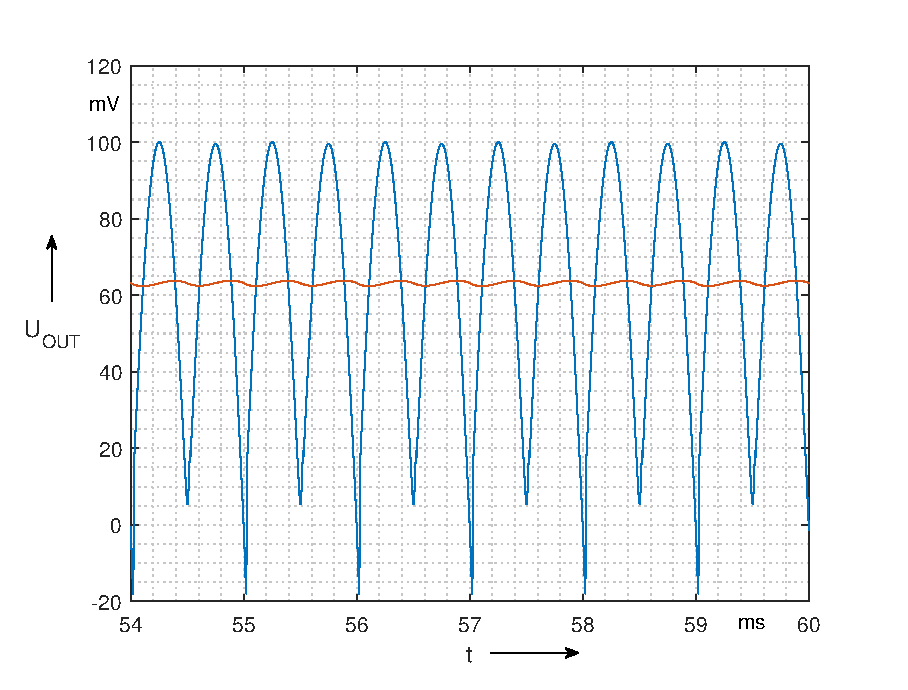
\includegraphics[width=\costumPicWidth]{Lab_3/Plots/Gleichrichter.eps}
    \caption{Simulationsergebnisse des Präzissionsgleichrichters}
    \label{fig:sim_Gleichrichter}
\end{figure}
\subsection{Ausarbeitungen}
%%%%%%%%%%%%%%%%%%%%%%%%%%%%%%%%%%%%%%%%%%%%%%%%%%%%%%%%%%%%%%%%%%%%%%%%%%%%%%%%%%%%%%%%%%%%%%%

\section{Single Supply Mikrofonverstärker mit LM358 und AD823}
\subsection{Aufgabenstellung}
Die Schaltung aus Abbildung \ref{fig:Mikrofon_Schaltung} soll bei einer Frequenz von $f=30Hz$ eine Verstärkung von $\nu = 40dB$ haben. 
Danach soll die Schaltung auf dem Steckbrett aufgebaut werden und ein Frequenzgang erfasst werden.

Auf einen Versuch mit Mikrofon und Lautsprecher wurde heuer wegen geringerer Laborzeit verzichtet. 

Nach Aufnahme des Amplitudengangs der Schaltung mit dem LM358 wird der Operationsverstärker mit dem pinkompatiblen AD823 ersetzt. Nun wird der Amplitudengang erneut aufgenommen. Diese beiden Amplitudengänge sind zu vergleichen. 
\begin{figure}[H]
    \centering
    \begin{circuitikz}[]
        \draw (0,0) node[op amp,yscale=-1] (opamp) {\scalebox{1}[-1]{$LM358$}};
        \draw (opamp.down) --++(0,0.5) node[vcc]{$V_{CC}$};
        \draw (opamp.up) --++(0,-0.5) node[vee]{$V_{EE}$};

        \draw (opamp.+) to[short] ++(-2,0) to[C=$C_1$,-o] ++(-2,0) node[left]{$U_{in}$};
        \draw (-3,0.5) to[R=$R_5$,*-] ++(0,2) node[vcc]{$V_{CC}$};
        \draw (-3,0.5) to[R=$R_4$,*-] ++(0,-2) node[ground]{};
        
        \draw (opamp.-) to[short] ++(-0.5,0)
            to[short] ++(0,-3)
            to[R=$R_2$] ++(0,-1.5)
            to[C=$C_3$] ++(0,-1.5) node[ground]{};
        \draw (opamp.out) to[short] ++(2,0)
            to[C=$C_2$,-o] ++(1.5,0) node[right]{$U_{out}$};
        \draw (3,0) to[R=$R_3$,*-] ++(0,-2) node[ground]{};
        \draw (2,0) to[short, *-] ++(0,-2.5)
            to[R=$R_1$,-*] ++(-3.7,0);
        \end{circuitikz}
    \caption{Mikrofonverstärker mit LM358 und AD823}
    \label{fig:Mikrofon_Schaltung}
 \end{figure}

\subsection{Messaufbau}
\subsection{Auslegung der Schaltung}
Die Schaltung soll bei $f=30Hz$ bereits eine Verstärkung von $\nu = -100$ aufweisen. Deswegen wurde die Grenzfrequenz der Schaltung mit $f_g=5Hz$ festgelegt. 
Dazu wurden ein paar der Widerstandswerte im Vorhinein angenommen. Mit dem damit resultierenden Tiefpass kann die Kapazität $C_1$ ausgelegt werden.
\begin{align}
    R_4=R_5 &= 100k\Omega \\
    R_{in} = \frac{R_4\cdot R_5}{R_4+ R_5} &= 50k\Omega \\
    C_1=\frac{1}{2\pi f_g R_{in}} = \frac{1}{2\cdot \pi \cdot 5\cdot50\cdot 10^3} &= 636.61nF \approx 2\cdot 330nF = 660nF
\end{align}
Durch die gegebene Verstärkung kann nun der Spannungsteiler $R_1$ und $R_2$ und die Kapazität $C_3$ ausgelegt werden. Die beiden hier verwendeten Widerstände sollten zwar ausreichend groß, jedoch nicht zu groß gewählt werden, da in diesem Bereich der Schaltung parasitäre Kapazitäten sehr leicht zu einem Tiefpassverhalten führen können. Besonders durch den Aufbau auf einem Steckbrett ist diese Schaltung anfällig dafür. 
\begin{align}
    R_1 &= 100k\Omega\\
    \nu = -100 &= -\frac{R_1}{R_2} \\
    R_2 = \frac{R_1}{\nu} &= 1k\Omega\\
    C_3=\frac{1}{2\pi f_g R_2} = \frac{1}{2\cdot \pi \cdot 5\cdot1\cdot 10^3} &= 31,813\mu F \approx 32\mu F
\end{align}
Da die Kapazität $C_2$ lediglich für eine kapazitive Kopplung der Schaltung sorgen soll, wurde ihr Wert willkürlich auf $C_2=100nF$ festgelegt. 

\begin{table}[H]
\centering
\caption{Bauteilwerte Mikrofonverstärker}
\label{tab:Bauteile_Mikrofonv}
\begin{tabular}{|l|r|r|}
\hline
\rowcolor[HTML]{C0C0C0} 
Bauteilname & \multicolumn{1}{l|}{\cellcolor[HTML]{C0C0C0}gewählter Wert} & \multicolumn{1}{l|}{\cellcolor[HTML]{C0C0C0}gemessener Wert} \\ \hline
$R_1$       & $100k\Omega$                                                & $99,491k\Omega$                                              \\ \hline
$R_2$       & $1k\Omega$                                                  & $1,0007k\Omega$                                              \\ \hline
$R_3$       & $100k\Omega$                                                & $98,098k\Omega$                                              \\ \hline
$R_4$       & $100k\Omega$                                                & $99,520k\Omega$                                              \\ \hline
$R_5$       & $100k\Omega$                                                & $98,422k\Omega$                                              \\ \hline
$C_1$       & $660nF$                                                     & $644nF$                                                      \\ \hline
$C_2$       & $100nF$                                                     & $98,5nF$                                                     \\ \hline
$C_3$       & $32\mu F$                                                   & $38,0\mu F$                                                  \\ \hline
\end{tabular}
\end{table}

\subsection{Messergebnisse}
\begin{figure}[H]
    \centering
    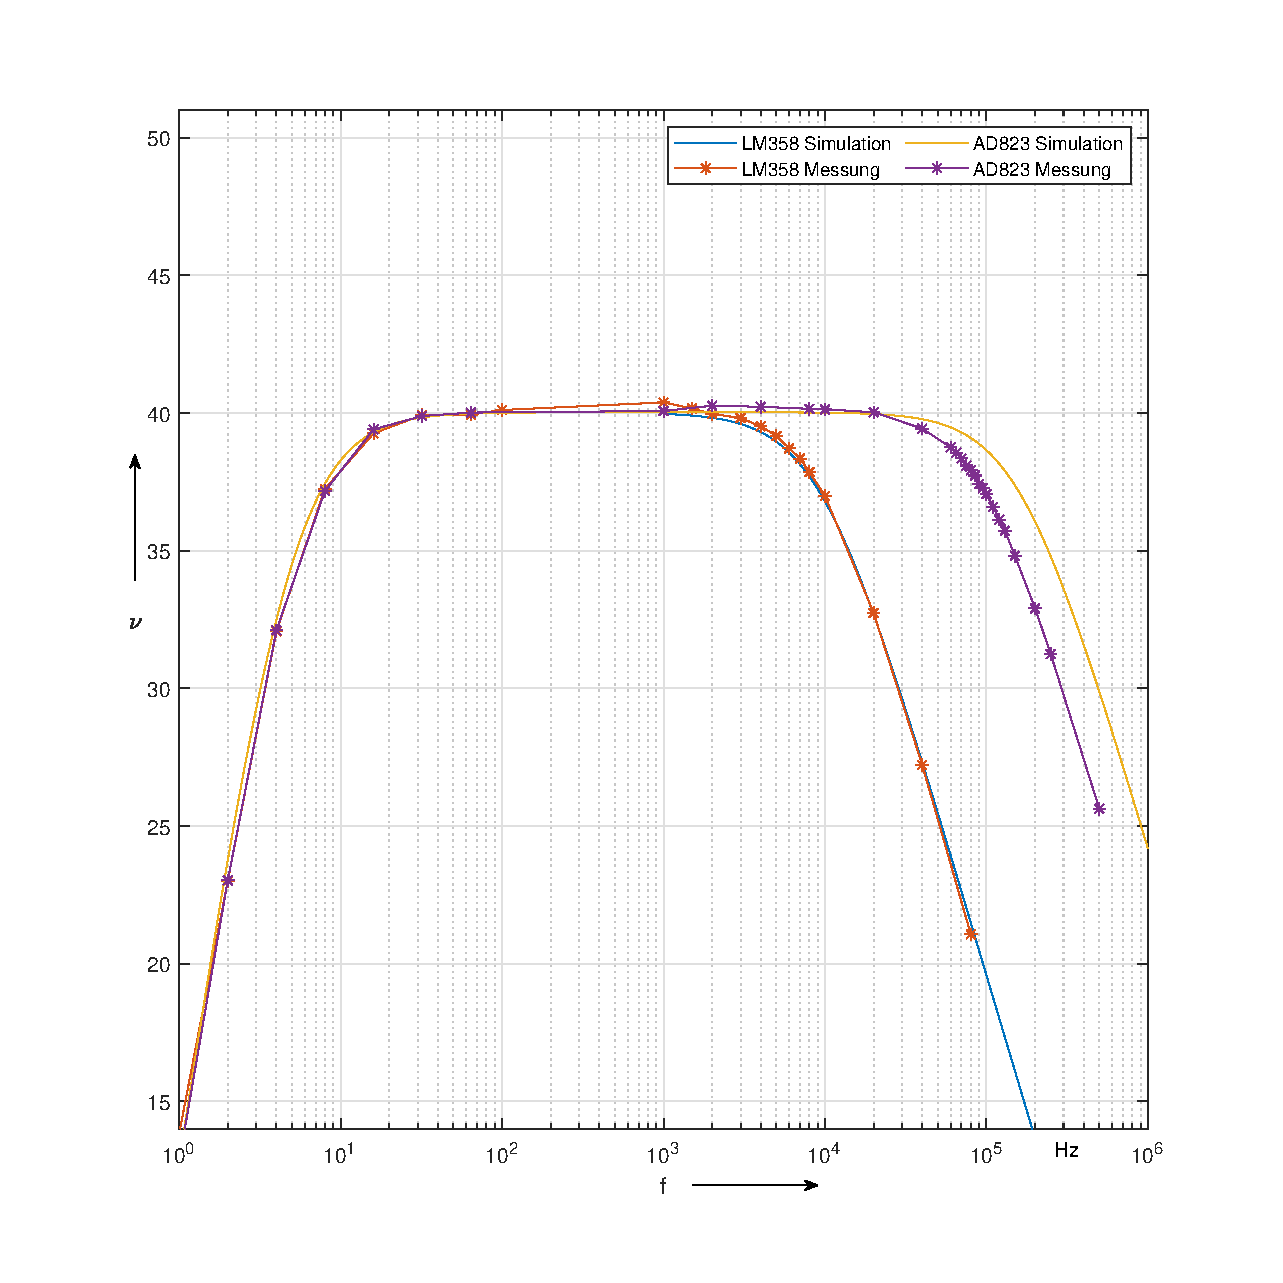
\includegraphics[width=\costumPicWidth]{Lab_3/Plots/Mikrofonverstaerker.eps}
    \caption{Vergleich der Amplitudengänge beim Mikrofonverstärker}
    \label{fig:Amplitudengang_Mikverstaerker}
\end{figure}
\subsection{Interpretation der Messergebnisse} 
Wie in Abbildung \ref{fig:Amplitudengang_Mikverstaerker} zu erkennen ist verhalten sich die real gemessenen Werte, sowie die Schaltungen mit beiden Operationsverstärkern nahezu ident. Die untere Grenzfrequenz liegt bei ungefähr $f_g=8Hz$, das führt dazu, dass bei 30Hz schon nahezu eine Verstärkung von $\nu = 40dB$ erreicht ist.

Bei der oberen Grenzfrequenz ist jedoch nun gut zu erkennen, dass der LM358 das Band bereits sehr viel früher begrenzt, als der AD823. Hier stimmen auch die simulierten Werte mit den gemessenen sehr gut überein. Das liegt vorrangig daran, dass parasitäre Kapauzäten bei solch geringen Frequenzen sehr wenig Einfluss auf die Schaltung haben.

Beim Vergleich der Simulation und der Messung der Schaltung mit dem AD823 ist eine deutlich höhere obere Grenzfrequenz auszumachen. Diese ist bei der gemessenen Schaltung etwas früher, was aber vermutlich an parasitären Kapazitäten im Steckbrett liegt. Dies musste ich während der Laboreinheit erfahren, da der erste Aufbau mit deutlich größeren Widerstandswerten aufgebaut wurde, um die Kapazität $C_3$ möglichst klein zu halten. Dabei erzeugt die Kapazität des Steckbrettes bereits bei $f_g=10^4Hz$ eine obere Grenzfrequenz. 

Für Audioanwendungen ist der AD823 gut geeignet, da der menschliche Hörbereich ungefähr von 16 - 20.000 Hz angegeben wird und die obere Grenzfrequenz bei diesem Verstärker jenseits der 50kHz ist.  Desweiteren beträgt die Samplerate bei MP3 ohnehin nur 44,2kHz, wobei nach dem Abtasttheorem nach Shannon - Nyquist Töne bis maximal 22,1 kHz wiederhergestellt werden können. Der LM358 ist jedenfalls nicht geeignet. Er zeigt bereits bei deutlich zu niedrigen Frequenzen ein Tiefpassverhalten und würde die Qualität des aufgenommenen Signals stark verringern. 
\subsection{Ausarbeitungen}

\section{Sallen-Key Tiefpassfilter}
\subsection{Aufgabenstellung}
Die Schaltung aus Abbildung \ref{fig:Sallen_key} ist auf eine $f_g=30Hz$ und auf eine Verstärkung von $\nu = +10$ auszulegen. Der Filter soll eine Butterworth Charakteristik aufweisen und mit dem Operationsverstärker AD823 auf dem Steckbrett aufgebaut werden.

Von dieser Schaltung ist während der Laboreinheit ein Bodediagramm aufzunehmen und die Sprungantwort zu messen.
\begin{figure}[H]
    \centering
    \begin{circuitikz}[]
        \draw (0,0) node[op amp,yscale=-1] (opamp) {\scalebox{1}[-1]{$AD823$}};
        \draw (opamp.down) --++(0,0.5) node[vcc]{$V_{CC}$};
        \draw (opamp.up) --++(0,-0.5) node[vee]{$V_{EE}$};
        
        \draw (opamp.+) to[short, -*] ++(-2,0)
            to[C=$C_2$] ++(0,-2) node[ground]{};
        \draw (opamp.+) to[short, -*] ++(-2,0)
            to[R=$R_2$] ++(-2,0)
            to[R=$R_1$,-o] ++(-2,0) node[left]{$U_{in}$};
        \draw (-5.25,0.5) to[short,*-] ++(0,2)
            to[C=$C_1$] ++(7.445,0)
            to[short] ++(0,-2.5)
            to[short] (opamp.out);
        \draw (opamp.out) to[short,-*] ++(1,0)
            to[R=$R_4$,-*] ++(0,-3)
            to[R=$R_3$] ++(0,-2) node[ground]{};
        \draw (2.2,-3) to[short] ++(-4,0)
            to[short] ++(0,2.5)
            to[short] (opamp.-);
        \draw (opamp.out) to[short,-o] ++(2,0) node[right] {$U_{out}$};
        \end{circuitikz}
    \caption{Sallen-key, Aktiver Tiefpass}
    \label{fig:Sallen_key}
 \end{figure}


\subsection{Auslegung}
Zur Auslegung dieser Schaltung ist die Übertragungsfunktion \cite[212]{10.5555/3158302} sehr hilfreich.

\begin{align}
    A(s) = \frac{A_0}{1+a_1s + b_1s^2}&=\frac{A_0}{1+\omega_c[C_1(R_1+R_2) + (1-A_0)R_1C_2]s + {\omega_C}^2R_1R_2C_1C_2s^2} \\
    \rm mit \it A_0 &= 1+ \frac{R_4}{R_3} 
\end{align}
Da dieser Filter eine Butterworth Charakteristik aufweisen soll, gilt für $a_1$ und $b_1$:

\begin{align}
    a_1 &= \sqrt{2} \\
    b_1 &= 1
\end{align}

Damit gilt: 
\begin{align}
    a_1 = \sqrt{2} &= \omega_c[C_1(R_1+R_2) + (1-A_0)R_1C_2] \label{eq:a1}\\
    b_1 = 1 &= {\omega_C}^2R_1R_2C_1C_2 \label{eq:b1}
\end{align}

Da im Labor wesentlich weniger verschiedene Kapazitätswerte als Widerstandswerte verfügbar sind, wurde mit der Wahl der Kapazitäten $C_1$ und $C_2$ begonnen. Im Falle der Auslegung einer Schaltung für den realen Einsatz sollte bei der Wahl dieser Kapazitäten auf geringe Toleranzen vom Absolutwert und bei Temperaturdrift wert gelegt werden. Im Labor waren ohnehin nur Kapazitäten mit $\pm10\%$ verfügbar. 

\begin{align}
    C_1 &= 100nF \\
    C_2 &= 330nF
\end{align}

Nach Umformen der Gleichungen \ref{eq:a1} und \ref{eq:b1} ergaben sich folgende Widerstandswerte:

\begin{align}
    R_1 &= 4,28k\Omega \\
    R_2 &= 198,4 k\Omega
\end{align}

\lstinputlisting[language = Matlab, caption=matlab Skript zur Auslegung des aktiven Filter]{Lab_3/auslegung_Sallen_key.m}

\subsection{Interpretation der Messergebnisse}
\begin{figure}[h]
    \centering
    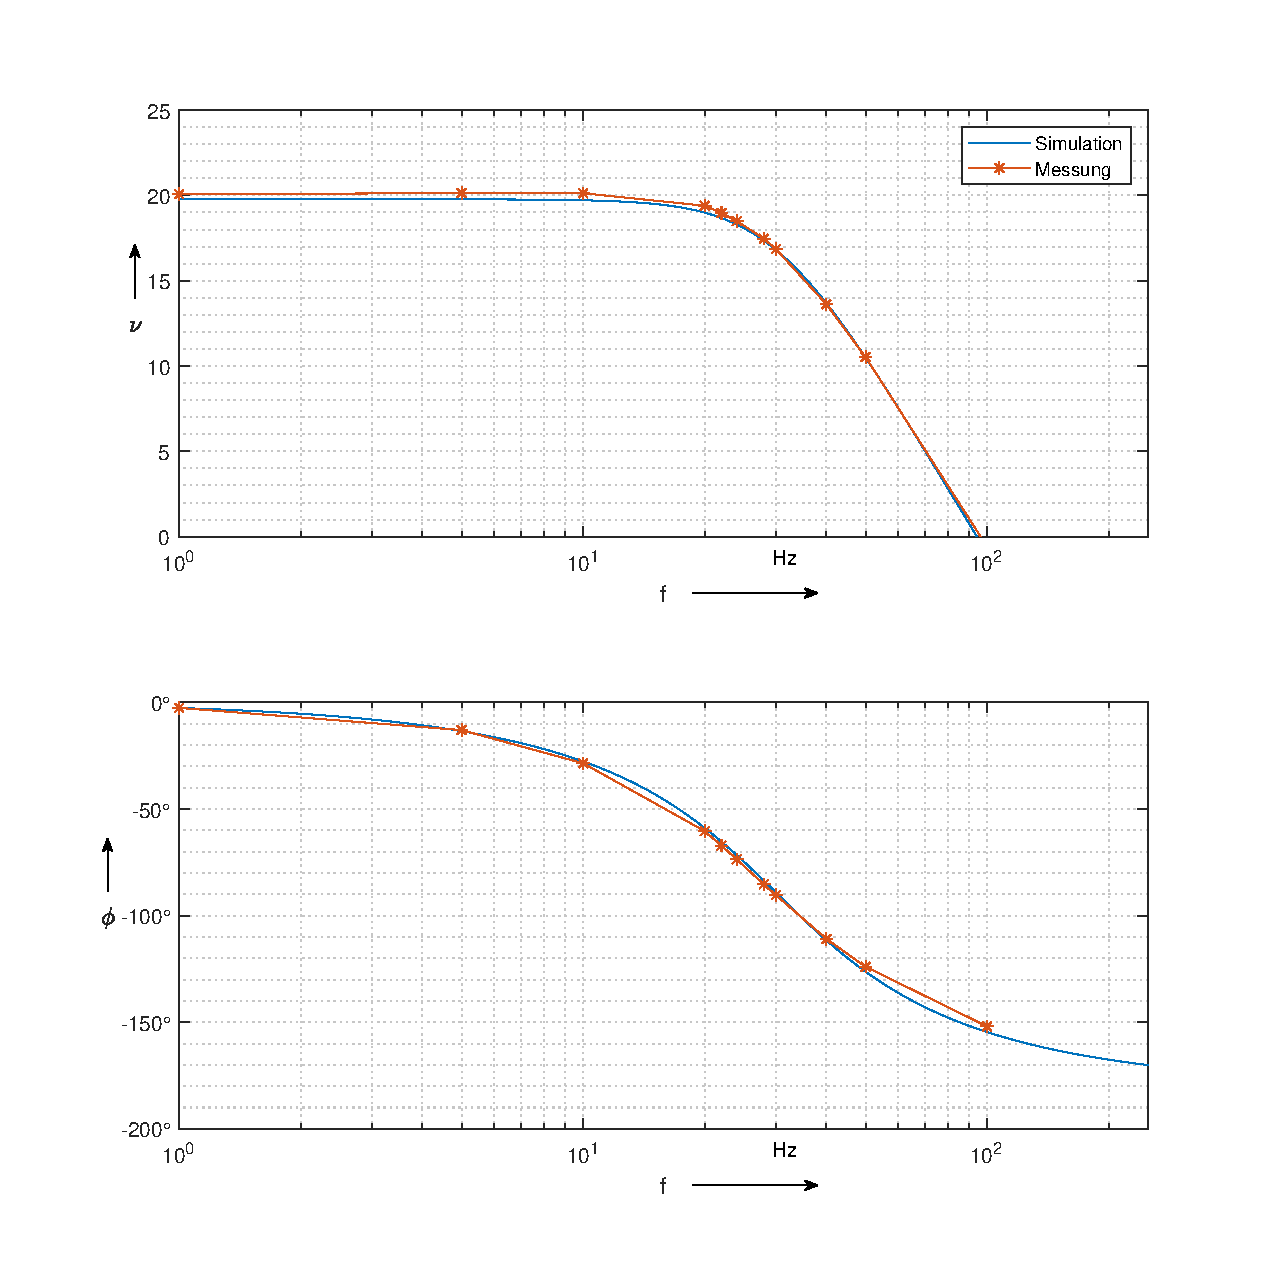
\includegraphics[width = \costumPicWidth]{Lab_3/Plots/sallen_key.eps}
    \caption{Bodediagramm aktiver Tiefpass 2. Ordnung}
    \label{fig:my_label}
\end{figure}